\section{Struttura delle memorie}
Le memorie hanno in generale diverse tipologie si strutture di controllo in base alla loro costruzione. La costruzione di una memoria non è universale, ciò è dovuto alla differente implementazione che tali memorie hanno a livello pratico. In una maniera più generale, le memorie possono essere suddivise in due categorie:
\begin{itemize}
    \item \textbf{Memorie statiche}: Le memorie statiche sono memorie che sono costruite tramite un insieme di transistor opportunamente collegati, non richiedono alcun tipo di sistema di refresh dei dati
    \item \textbf{Memorie dinamiche}: Le memorie dinamiche sono memorie che funzionano mediante effetti capacitivi. Pertanto richiedono che vi sia implementato un opportuno sistema di refresh
\end{itemize}
Tali memorie vengono utilizzate in base all'ambito di applicazione e alla velocità richiesta. Tali argomentazioni saranno affrontate nei capitoli appositi

\subsection{Memorie Dinamiche}
Le memorie dinamiche sono memorie che utilizzano gli effetti capacitivi per memorizzare l'informazione. Un esempio semplice di cella di memorizzazione di una memoria dinamica è osservabile alla figura [\ref{img:mem-dinamica}]. Come possiamo notare, la memorizzazione dipende fortemente dalla carica di un condenzatore, che quindi richiede di dover implementare un meccanismo di refresh. Tale meccanismo di refresh può essere fatto in vari modi, in base alle modalità di accesso ai dati della specifica memoria.

\begin{figure}
    \centering
    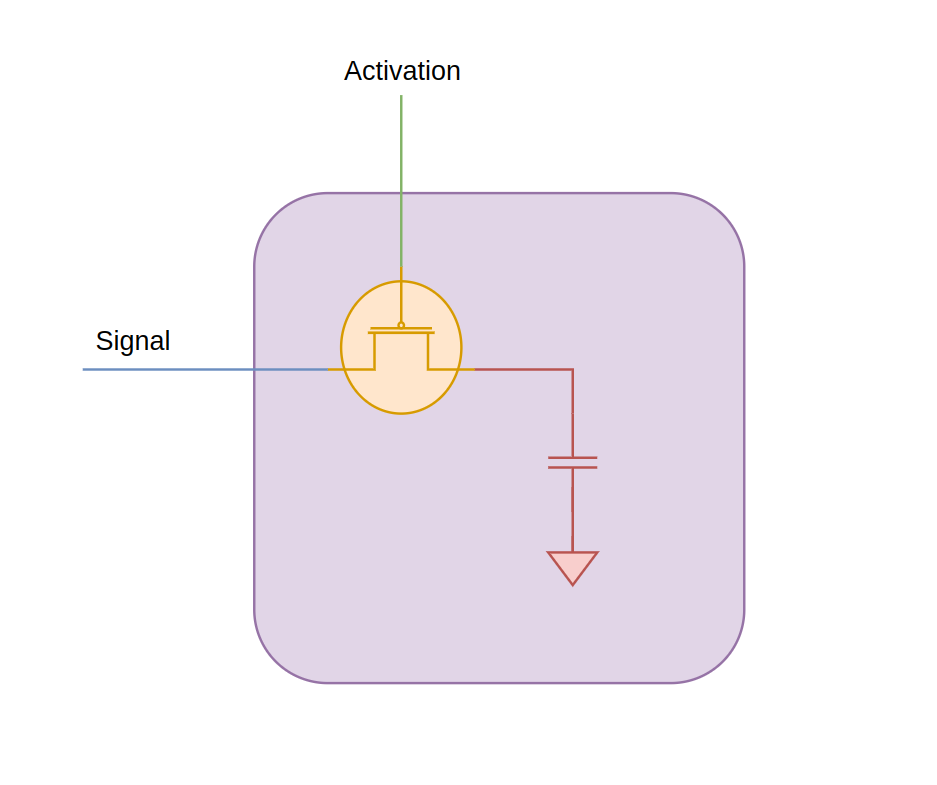
\includegraphics[width=.3\textwidth]{img/DRAM-CELL.png}
    \caption{Cella di una memoria DRAM}\label{img:mem-dinamica}    
\end{figure}
Le memorie, oltre alla cella, sono composte da altri componenti di "gestione". Tali elementi sono:
\begin{itemize}
    \item \textbf{Decoder}: Passa dall'indirizzo inserito alla linea (riga) da andare ad attivare
    \item \textbf{Multiplexer}: Permette di selezionare a quale elemento si sta facendo riferimento in fase di lettura (Selezione della colonna)
    \item \textbf{Demultiplexer}: Permette di selezionare un elemento da andare a modificare, spendibile particolarmente nella fase di scrittura dell'elemento (Selezione della colonna su cui andare a scrivere)
    \item \textbf{Sistema di refresh}: Sistema che permette di "rinfrescare" i dati che sono presenti nella memoria, che ad intervalli di tempo esegue il refresh. Tale condizione, quindi, presuppone un disattivamento della memoria per qualche periodo di tempo, sinonimo di lentezza aggiunta
    \item \textbf{Contatori}: Contatori per ricordare, in fase di refresh, l'indice della riga da rinfrescare e il tempo da attendere prima di effettuare un nuovo rinfresco
\end{itemize}

Il funzionamento principale di una memoria DRAM (che possiamo vedere come una sorta di modello di programmazione) è pilotata da 2 principali indirizzi (provenienti dal singolo indirizzo fisico), che ne permettono di selezionare la riga e la colonna. 
Tali registri sono chiamati \textbf{RAS}(Row Address Strobe o Row Address Select) e \textbf{CAS}(Column Address Strobe o Column Address Select), il loro preciso valore viene estratto dalla divisione dell'indirizzo FISICO posto nell'apposito ingresso indirizzi (dell'interfaccia di memoria dall'esterno). La memoria parte col selezionare un intera riga, che, passa in prima battuta tra una serie di amplificatori e poi, tramite il CAS, si va a selezionare il dato desiderato. Tale meccanismo di funzionamento, permette alla memoria, ad ogni lettura di una particolare riga, di poterne effettuare anche il redresh. Tale refresh, però, può essere effettuato anche per determinati tempi di delay (immaginiamo se una riga non viene mai acceduta, c'è bisogno di refresharla prima che i dati all'interno dei condensatori vadano persi), la fase di refresh avviene regolarmente, la pausa tra una fase di refresh e l'altra viene effettuata tramite l'utilizzo di un apposito contatore, che ogni N-impulsi di clock, dove N è il numero di impulsi di clock per scandire un determinato tempo, tale tempo viene deciso in base al tempo di decadenza che caratterizza i condensatori utilizzati per la costruzione della memoria. Pertanto, tali memorie, per effettuare un operazione, nel peggiore dei casi, devono far aspettare almeno il tempo di refresh e poi accedere allo specifico dato. Pertanto tale tecnologia non è tanto utilizzata nelle memorie cache, quando nelle RAM. Difatti ad oggi le RAM sono realizzate principalmente con strutture di tipo dinamico.
Oltre ad un tipo di vantaggio fisico, vi è anche un grande vantaggio logico, utilizzando una tecnologia di tipo dinamico per la realizzazione delle RAM, il passaggio di dati tra la cache e la memoria avviene più velocemente, poichè tramite un sigolo RAS, ottengo tutta una riga di informazioni che possono essere trasmesse direttamente in cache (tramite le sole modifiche del CAS). In questo modo i trasferimenti tra la memoria cache e quella RAM risultano più ottimizzati e veloci.
Per ottimizzare al meglio questo processo, si potrebbe pensare di ottimizzarlo tramite azioni che possono avvenire su fronti di clock differenti, tutte queste operazioni, però, richiedono un sistema puramente sincrono, mentre nel caso delle memorie il funzionamento dev'essere per forza semi-sincrono. Per la memoria cache la semi-sincronicità è verificata per via della presenza dei cache miss (richiedono di dover prelevare dati da altre memorie esterne), mentre nel caso delle memorie dinamiche è dovuta alla presenza della fase direfresh, poichè, se arriva una richiesta durente la fase di refresh, questa viene fatta attendere (poichè la fase di refresh ha maggiore priorità), per poi essere adeguatamente servita. 

\subsection{Memorie Statiche}
Le memorie statiche sono memorie realizzate principalmente con strutture di transistor Mosfet collegati in un certo modo. Una volta registrato il dato all'interno di tali celle, esso rimane "intrappolato" nella rete logica associata. La struttura di una cella semplice di memoria statica è quella visualizzabile alla figure [\ref{img:memoria-statica}]

Tale tipologia di memoria è impiegata principalmente nella realizzazione di memorie cache, poichè risulta altamente veloce ed efficente. Anche se richiede una complessa gestione dell'hardware (conservazione dello stato di ossido di silicio), la velocità ne compensa, questo poichè la memoria sarà sempre disponibile per il prelievo dei dati senza dover affrontare alcun tipo di refresh, come nel caso delle specifiche memorie dinamiche

\begin{figure}
    \centering
    \subfloat[][\emph{Memoria CMOS a 6 transistor}]{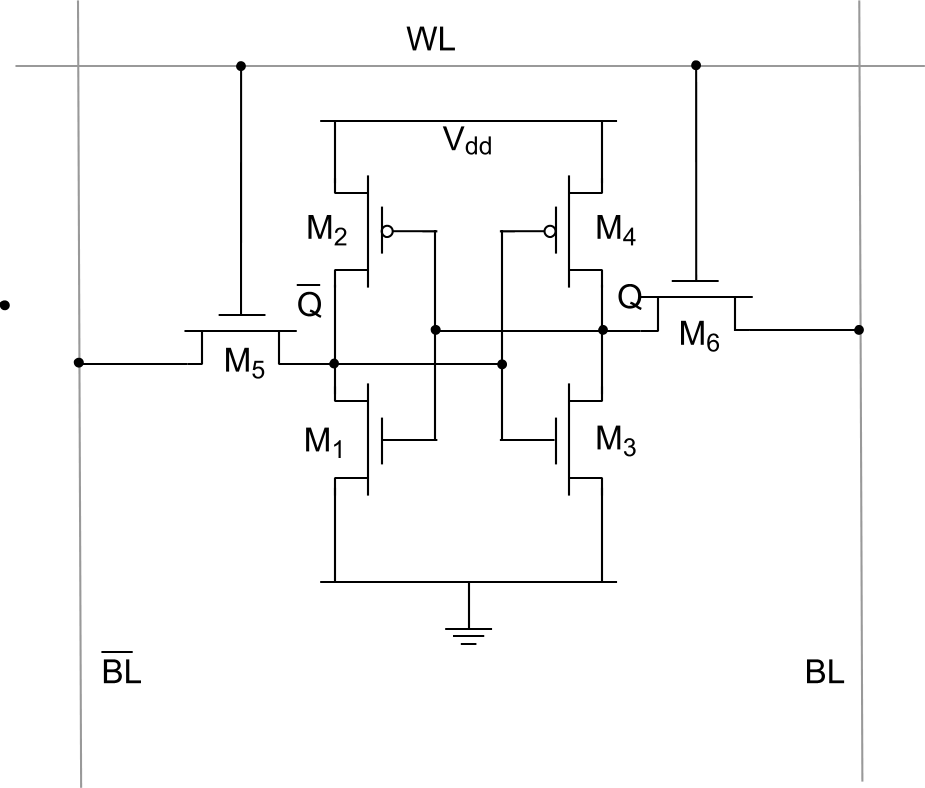
\includegraphics[width=.45\textwidth]{img/SRAM.png}}\quad
    \subfloat[][\emph{Struttura logica}]{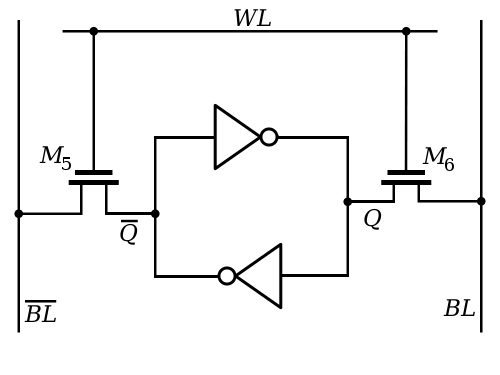
\includegraphics[width=.45\textwidth]{img/SRAM-2.png}}
    \caption{Struttura CMOS di una cella di memoria statica semplice}\label{img:memoria-statica}
\end{figure}
